\documentclass[12pt]{article}
\usepackage[a4paper, margin=1in]{geometry}
\usepackage{tikz}
\usepackage{graphicx}

% Both idBox4.pdf (Plom's student ID box) and choice4box.pdf must be
% in the same folder as this .tex file when compiling.
\graphicspath{{./}}

\pagestyle{empty}

% -----------------------------------------------------------------------
% Corner fiducial markers for our OMR alignment (same as other templates)
% -----------------------------------------------------------------------
\newcommand{\fiducials}{%
  \begin{tikzpicture}[remember picture, overlay]
    \fill[black]
      ([xshift=15mm,  yshift=-20mm]current page.north west) rectangle
      ([xshift=20mm,  yshift=-15mm]current page.north west);
    \fill[black]
      ([xshift=-20mm, yshift=-20mm]current page.north east) rectangle
      ([xshift=-15mm, yshift=-15mm]current page.north east);
    \fill[black]
      ([xshift=15mm,  yshift=15mm]current page.south west) rectangle
      ([xshift=20mm,  yshift=20mm]current page.south west);
    \fill[black]
      ([xshift=-20mm, yshift=15mm]current page.south east) rectangle
      ([xshift=-15mm, yshift=20mm]current page.south east);
  \end{tikzpicture}%
}

\begin{document}

% =====================================================================
% PAGE 1 — Cover / Student ID page
% Plom expects the student ID box on the first page.
% Plom will stamp its QR codes on this page automatically.
% =====================================================================
\fiducials
\vspace*{1.5cm}

\begin{center}
  {\LARGE Math 101 — Midterm Exam}\\[0.5cm]
  {\large Please write your student ID in the box below.}
\end{center}

\vspace{0.8cm}
\begin{center}
  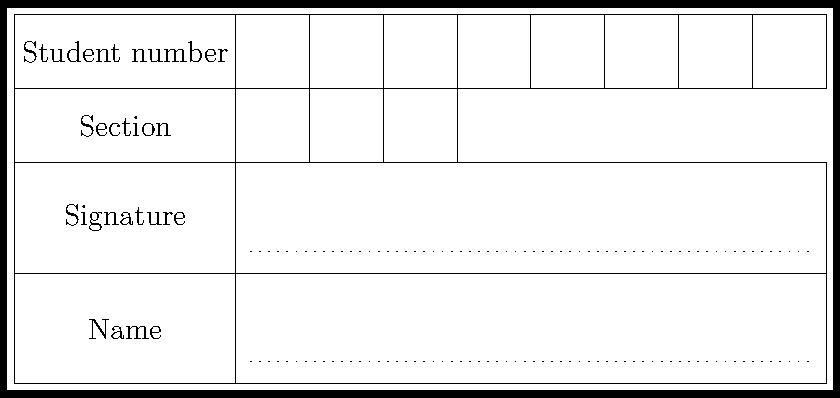
\includegraphics[width=0.85\textwidth]{idBox4}
\end{center}

\vspace{1cm}
\noindent\textbf{Instructions:}
\begin{itemize}
  \item For each question, circle the letter of your chosen answer inside the box.
  \item Use a dark pen or pencil.
  \item Do not write outside the answer boxes.
\end{itemize}

\newpage

% =====================================================================
% PAGE 2 — MCQ answer page
% Our OMR server will read this page.
% Plom will also stamp QR codes here.
% =====================================================================
\fiducials
\vspace*{1cm}

\begin{center}
  {\Large Answer Sheet}
\end{center}

\vspace{1cm}

% ---- Question 1 ----
\noindent\textbf{Question 1:} Which of the following is a prime number?

\vspace{0.3cm}
\noindent
\includegraphics[width=0.85\textwidth]{choice4box}

\vspace{0.8cm}

% ---- Question 2 ----
\noindent\textbf{Question 2:} What is $2^{10}$?

\vspace{0.3cm}
\noindent
\includegraphics[width=0.85\textwidth]{choice4box}

\vspace{0.8cm}

% ---- Question 3 ----
\noindent\textbf{Question 3:} Which sorting algorithm has worst-case $O(n \log n)$?

\vspace{0.3cm}
\noindent
\includegraphics[width=0.85\textwidth]{choice4box}

\end{document}
